
%%%%%%%%%%%%%%%%%%%%%%%%%%%%%%%%%%%%%%%%%
% Short Sectioned Assignment LaTeX Template Version 1.0 (5/5/12)
% This template has been downloaded from: http://www.LaTeXTemplates.com
% Original author:  Frits Wenneker (http://www.howtotex.com)
% License: CC BY-NC-SA 3.0 (http://creativecommons.org/licenses/by-nc-sa/3.0/)
%%%%%%%%%%%%%%%%%%%%%%%%%%%%%%%%%%%%%%%%%

% \documentclass[paper=a4, fontsize=11pt]{scrartcl} % A4 paper and 11pt font size
\documentclass[11pt, a4paper, oneside]{book}
\usepackage[T1]{fontenc} % Use 8-bit encoding that has 256 glyphs
\usepackage[utf8]{inputenc}
\usepackage{fourier} % Use the Adobe Utopia font for the document - comment this line to return to the LaTeX default
\usepackage{listings} % para insertar código con formato similar al editor
\usepackage[spanish, es-tabla]{babel} % Selecciona el español para palabras introducidas automáticamente, p.ej. "septiembre" en la fecha y especifica que se use la palabra Tabla en vez de Cuadro
\usepackage{url} % ,href} %para incluir URLs e hipervínculos dentro del texto (aunque hay que instalar href)
\usepackage{graphics,graphicx, float} %para incluir imágenes y colocarlas
\usepackage[gen]{eurosym} %para incluir el símbolo del euro
\usepackage{cite} %para incluir citas del archivo <nombre>.bib
\usepackage{enumerate}
\usepackage{hyperref}
\usepackage{graphicx}
\usepackage{tabularx}
\usepackage{booktabs}
\usepackage{indentfirst}
\usepackage[table,xcdraw]{xcolor}
\hypersetup{
	colorlinks=true,	% false: boxed links; true: colored links
	linkcolor=black,	% color of internal links
	urlcolor=cyan		% color of external links
}
\renewcommand{\familydefault}{\sfdefault}
\usepackage{fancyhdr} % Custom headers and footers
\pagestyle{fancyplain} % Makes all pages in the document conform to the custom headers and footers
\fancyhead[L]{} % Empty left header
\fancyhead[C]{} % Empty center header
\fancyhead[R]{Cecilia Merelo Molina} % My name
\fancyfoot[L]{} % Empty left footer
\fancyfoot[C]{} % Empty center footer
\fancyfoot[R]{\thepage} % Page numbering for right footer
%\renewcommand{\headrulewidth}{0pt} % Remove header underlines
\renewcommand{\footrulewidth}{0pt} % Remove footer underlines
\setlength{\headheight}{13.6pt} % Customize the height of the header

\usepackage{titlesec, blindtext, color}
\definecolor{gray75}{gray}{0.75}
\newcommand{\hsp}{\hspace{20pt}}
\titleformat{\chapter}[hang]{\Huge\bfseries}{\thechapter\hsp\textcolor{gray75}{|}\hsp}{0pt}{\Huge\bfseries}
\setcounter{secnumdepth}{4}
\usepackage[Lenny]{fncychap}


\begin{document}
	% Plantilla portada UGR
	\begin{titlepage}
\newlength{\centeroffset}
\setlength{\centeroffset}{-0.5\oddsidemargin}
\addtolength{\centeroffset}{0.5\evensidemargin}
\thispagestyle{empty}

\noindent\hspace*{\centeroffset}\begin{minipage}{\textwidth}

\centering

\includegraphics[width=0.9\textwidth]{logos/logo_ugr.jpeg}\\[1.4cm]

\textsc{ \Large TRABAJO FIN DE GRADO\\[0.2cm]}
\textsc{ GRADO EN INGENIERIA INFORMATICA}\\[1cm]

{\Huge\bfseries Título \\}
\noindent\rule[-1ex]{\textwidth}{3pt}\\[3.5ex]
{\large\bfseries Subtítulo }
\end{minipage}

\vspace{2.5cm}
\noindent\hspace*{\centeroffset}
\begin{minipage}{\textwidth}
\centering

\textbf{Autor}\\ {Cecilia Merelo Molina}\\[2.5ex]
\textbf{Director}\\ {Juan Julián Merelo Guervós}\\[2cm]

\includegraphics[width=0.3\textwidth]{logos/etsiit_logo.png}\\[0.1cm]
\textsc{Escuela Técnica Superior de Ingenierías Informática y de Telecomunicación}\\
\textsc{---}\\
Granada, Junio de 2021
\end{minipage}
\end{titlepage}


	% Plantilla prefacio UGR
	\thispagestyle{empty}

\begin{center}
{\large\bfseries Título \\ Subtítulo }\\
\end{center}
\begin{center}
Nombre Del Estudiante\\
\end{center}

%\vspace{0.7cm}

\vspace{0.5cm}
\noindent{\textbf{Palabras clave}: \textit{software libre}
\vspace{0.7cm}

\noindent{\textbf{Resumen}\\
	

\cleardoublepage

\begin{center}
	{\large\bfseries Same, but in English}\\
\end{center}
\begin{center}
	Student's name\\
\end{center}
\vspace{0.5cm}
\noindent{\textbf{Keywords}: \textit{open source}, \textit{floss}
\vspace{0.7cm}

\noindent{\textbf{Abstract}\\


\cleardoublepage

\thispagestyle{empty}

\noindent\rule[-1ex]{\textwidth}{2pt}\\[4.5ex]

D. \textbf{Tutora/e(s)}, Profesor(a) del ...

\vspace{0.5cm}

\textbf{Informo:}

\vspace{0.5cm}

Que el presente trabajo, titulado \textit{\textbf{Chief}},
ha sido realizado bajo mi supervisión por \textbf{Estudiante}, y autorizo la defensa de dicho trabajo ante el tribunal
que corresponda.

\vspace{0.5cm}

Y para que conste, expiden y firman el presente informe en Granada a Junio de 2018.

\vspace{1cm}

\textbf{El/la director(a)/es: }

\vspace{5cm}

\noindent \textbf{(nombre completo tutor/a/es)}

\chapter*{Agradecimientos}






	% Índice de contenidos
	\newpage
	\tableofcontents

	% Índice de imágenes y tablas
	\newpage
	\listoffigures

	% Si hay suficientes se incluirá dicho índice
	\listoftables 
	\newpage

	% Introducción 
	\chapter{Introducción}

\section{Motivación}

A principios de este año leí el conocido libro de Aldous Huxley: Un mundo feliz. La novela es una
distopía que describe el desarrollo en tecnología reproductiva, cultivos humanos e hipnopedia y el manejo de las
emociones por medio de drogas. La población se ordena en \textbf{castas}, asignadas desde el nacimiento, donde cada uno
sabe y acepta su lugar en la sociedad. La guerra y la pobreza han sido erradicadas, y todos son permanentemente
felices.

Cuando hablamos de algoritmos genéticos nuestro objetivo es alcanzar la solución óptima de un problema, y este libro describe el 
proceso mediante el cual han alcanzado la raza humana perfecta. Por tanto el objetivo final de este trabajo es desarrollar
un algoritmo genético basándonos en el proceso de fecundación del libro y comparar su comportamiento con otros algoritmos. Además
investiga cómo la división en castas afecta la diversidad en la población.

\section{Objetivos del trabajo}

\begin{enumerate}
    \item Adaptar la división en castas y el concepto de raza humana perfecta descrita en el libro a un algoritmo genético.
    \item Investigar cómo afecta la división en castas a la diversidad.
    \item Desarrollar el algoritmo siguiendo metodologías ágiles
    \item Demostrar que el lenguaje de programación Julia es buena opción para el desarrollo de algoritmos
\end{enumerate}

\section{Conceptos generales}

En el libro se describe cómo se alcanza esta raza humana perfecta mediante una \"cadena de montaje\", con
varias fases. Esto lo reflejaremos mediante un algoritmo evolutivo generacional con los operadores de selección, cruce, mutación
y reemplazamiento. El proceso comienza en la \textbf{\textit{Sala de Fecundación}}, aquí se crean los óvulos y se fecundan. Una
vez \textit{fecundados} los óvulos pasan a las incubadoras, donde se decide la \textit{casta} a la que pertenecerá cada individuo:

\begin{itemize}
    \item \textbf{Alphas}:
        \begin{itemize}
            \item Libro: son los más inteligentes, a este grupo pertenece la élite. Tienen responsabilidades y son
            los que tienen la capacidad de tomar decisiones.
            \item Implementación: se reproducirán sólo entre ellos, pasarán por todos los operadores del algoritmo.
        \end{itemize}
    \item \textbf{Betas}: 
        \begin{itemize}
            \item Libro: son menos inteligentes que los anteriores y su función principal se reduce a tareas
            administrativas.
            \item  Implementación: el cruce sólo se realiza con individuos Alpha
        \end{itemize}
    \item \textbf{Gammas}: 
        \begin{itemize}
            \item Libro: son los empleados subalternos, cuyas tareas requieren de habilidad. Son expertos en tareas repetitivas
            \item Implementación: los individuos de esta casta solo tendrán mutación, por búsqueda local.
        \end{itemize}
    \item \textbf{Castas Bajas}: sólo tendrán el operador de mutación por segmento fijo, sin búsqueda local. A este sector pertenecen:
        \begin{itemize}
            \item \textbf{Deltas}:a este grupo pertenecen los empleados de los anteriores.
            \item \textbf{Epsilones}: es la casta inferior, a ella pertenecen los empleados para trabajos arduos.
        \end{itemize}
\end{itemize}

Con esta estructura en mente la metaheurística se divide en las siguientes fases:

\begin{itemize}
    \item \textbf{Sala de Fecundación}: los individuos son creados de manera totalmente aleatoria. Tantos individuos
    como indique un parámetro \textit{I}.
    \item \textbf{Sala de incubación}: en esta fase realizamos la división en castas. Se hará basándonos en el valor de
    la función objetivo del individuo. Además cada casta tendrá un porcentaje diferente de la población.
    \item \textbf{Evolución de las castas}: cada casta seguirá un proceso de evolución diferente como ya se 
    ha mencionado.
\end{itemize}

El tamaño de la población descenderá cuanto más alta sea la casta.


Este proyecto es software libre, y está liberado con la licencia \cite{gplv3}.

	% Descripción del problema y hasta donde se llega
	\chapter{Descripción del problema y caracterización de la solución}

En este capítulo se describe el problema cuya solución se quiere abordar en este trabajo. Primero se analiza la naturaleza del algoritmo que
se quiere implementar, luego se describe la metaheurística desarrollada, para acabar con los casos de uso que se han ido 
implementando hasta conseguir la funcionalidad completa.

\section{Descripción}

En 2019, para la asignatura de metaheurísticas de la Universidad de Granada \cite{merelo_molina_2021} se propuso inventar una 
metaheurística. En ese momento acababa de leer el libro ``Un Mundo feliz`` de Aldous Huxley, así que decidí adaptar el proceso de 
optimización de la población humana que describe el libro a un algoritmo evolutivo. A lo largo del desarrollo se me presentaron varios retos.
El primero fue el lenguaje escogido; lo desarrollé en Python, un lenguaje caracterizado por su fácil sintaxis pero su deficiencia de
velocidad. Cada ejecución del problema llevaba horas, por lo que se hacía muy difícil de ejecutar y analizar. El
segundo fue la optimización de los parámetros; el algoritmo quedaba estancado en óptimos locales. Estos problemas son 
los que se quieren abordar en el desarrollo de este trabajo.

Como se ha mencionado en la sección anterior, se quiere desarrollar una metaheurística inspirada por un libro. Pero no solo interesa
el poder adaptar el proceso descrito en el libro a una metaheurística. También se busca que la metaheurística pueda ser
usada fácilmente por la comunidad, que su implementación sea extensible y mantenible, y además fácil de analizar. Para conseguirlo
se desarrollará una biblioteca que sea adaptable al problema a resolver, donde los parámetros iniciales sean 
indicados por la persona que use el algoritmo; parámetros como la función de fitness, tamaño de la población inicial,
dimensión del cromosoma y rango de búsqueda

\section{Naturaleza del algoritmo}

Como se ha mencionado, el algoritmo está basado en el proceso de optimización de la población humana que describe el libro 
a un algoritmo evolutivo, por tanto, estamos hablando de un algoritmo basado en la evolución de una población, así que seguirá 
la estructura de los algoritmos evolutivos, más en concreto, un \emph{algoritmo genético}. Se trata de un algoritmo 
genético ya que es un algoritmo de optimización de búsqueda inspirado en los procesos de Evolución Natural y
Evolución Genética.

Siguiendo la definición dada por Goldberg \cite{goldberg89}, "los Algoritmos Genéticos son algoritmos de búsqueda
basados en la mecánica de selección natural. Combinan la supervivencia del más apto entre estructuras de secuencias con un intercambio de 
información estructurado, aunque aleatorizado, para construir así un algoritmo de búsqueda que tenga algo de las genialidades de las 
búsquedas humanas". En resumen, estos algoritmos reflejan el proceso de la selección natural. Forman parte del grupo de 
los \emph{algoritmos evolutivos}. El proceso está compuesto de 4 fases:

\begin{itemize}
    \item Creación de la población inicial: el proceso comienza con un conjunto de individuos llamado \emph{Población}. Cada individuo
    representa una solución del problema a resolver. Cada individuo se caracteriza por una serie de parámetros llamados
    \emph{genes}. Los genes se unen para formar un \emph{Cromosoma}. Estos se crean en la primera generación. La población del 
    resto de generaciones serán evoluciones de esta población inicial.
    \item Selección: la idea de la fase de selección es seleccionar los individuos más adecuados para que pasen sus
    genes a las siguientes generaciones. Los individuos con mejor valor de fitness son los que tienen más posibilidades
    de ser seleccionados para la reproducción.
    \item Cruce: produce un nuevo individuo por cada pareja de padres, seleccionando de uno de ellos un segmento
    continuo de características y copiándolo en la descendencia. Los genes que quedan por asignar en la descendencia
    combinan de manera uniforme características de los dos padres.
    \item Mutación: en los hijos, algunos de los genes pueden ser sometidos a mutación, es decir, alguno de sus genes
    serán cambiados.
\end{itemize}

Además de las fases también se debe definir una \emph{condición de parada} y una \emph{función de fitness}. La 
condición de parada sirve para que el algoritmo finalice si la población converge, es decir, si no produce hijos 
que sean diferentes con respecto a las generaciones anteriores, o si alcanza la solución. La función de fitness
determina cómo de adecuado es un individuo, esto es, la probabilidad de que un individuo sea seleccionado para 
la reproducción depende de este valor. Por tanto, para alcanzar la solución a un problema se parte de un conjunto 
inicial de individuos, llamado \textit{población inicial}, generado de manera aleatoria. Cada uno de estos 
individuos representa una posible solución al problema. Estos individuos van pasando por los diferentes operadores y 
evolucionando en cada generación.

En el caso del algoritmo propuesto en este trabajo (\emph{Algoritmo Feliz}) la población evolucionará siguiendo un proceso 
inspirado por los distintos procesos descritos en el libro de Aldous Huxley. El proceso propuesto se describe con mayor detalle
en la sección \ref{sect: description}. Al usar como guía los procesos descritos en el libro quiere decir que se está desarrollando 
una metaheurística. Esta se trata de un método de alto nivel, independiente del problema, que proporciona una serie de guías o 
estrategias para desarrollar algoritmos de optimización heurísticos \cite{metaheuristics_def}. Muchas metaheurísticas
están inspiradas en la naturaleza \cite{Molina2020ComprehensiveTO}. Por ejemplo, la optimización basada en colonias de
hormigas que imita la manera en la que las hormigas se comportan cuando viajan a una fuente de comida, y cómo se 
comunican unas con otras a través de feromonas. 

Normalmente las metaheurísticas se usan en problemas de optimización por varias razones:
\begin{itemize}
    \item Encuentran maneras de ir de una solución a otra mejor sin tener por qué considerar todas las posibles combinaciones. 
    \item Pueden evitar quedarse estancadas en mínimos locales porque usan aleatoriedad.
\end{itemize}

En conclusión, se va a desarrollar una metaheurística basada en el proceso de fecundación y la división en castas descrita en el 
libro de A. Huxley.

\section{Descripción de la metaheurística desarrollada} \label{sect: description}

El libro describe cómo se alcanza esta raza humana perfecta mediante una ``cadena de montaje``, con varias fases. Esto lo 
reflejaremos mediante un algoritmo evolutivo generacional con los operadores de selección, cruce, mutación y reemplazamiento. 
El proceso comienza en la \textbf{\textit{Sala de Fecundación}}; aquí se crean los óvulos y se fecundan. Una vez \textit{fecundados}
los óvulos pasan a las incubadoras, donde se decide la \textit{casta} a la que pertenecerá cada individuo. Huxley describe 
como a los Alfas y los Betas se les suministra una gran cantidad de nutrientes y hormonas durante la incubación. Mientras que las 
castas bajas, Gamma, Delta y Epsilon son privadas de estos elementos necesarios para el desarrollo. Para imitar esta
 ``falta de nutrientes``, en el algoritmo a desarrollar privaremos a las castas bajas de operadores, solo mutarán. Con esto
 pretendo avanzar el objetivo de mantener la diversidad alta durante toda la ejecución del algoritmo. 
 Las castas se implementarán de la siguiente manera: 

\begin{itemize}
    \item \textbf{Alfas}:
        \begin{itemize}
            \item Libro: son los más inteligentes, a este grupo pertenece la élite. Tienen responsabilidades y son
            los que tienen la capacidad de tomar decisiones.
            \item Implementación: se reproducirán solo entre ellos, pasarán por todos los operadores del algoritmo.
        \end{itemize}
    \item \textbf{Betas}: 
        \begin{itemize}
            \item Libro: son menos inteligentes que los anteriores y su función principal se reduce a tareas
            administrativas.
            \item  Implementación: el cruce sólo se realiza con individuos Alpha.
        \end{itemize}
    \item \textbf{Gammas}: 
        \begin{itemize}
            \item Libro: son los empleados subalternos, cuyas tareas requieren de habilidad. Son expertos en tareas repetitivas
            \item Implementación: los individuos de esta casta solo tendrán mutación por búsqueda local.
        \end{itemize}
    \item \textbf{Castas Bajas}: sólo tendrán el operador de mutación por segmento fijo, sin búsqueda local. A este sector pertenecen:
        \begin{itemize}
            \item \textbf{Deltas}:a este grupo pertenecen los empleados de los anteriores.
            \item \textbf{Epsilones}: es la casta inferior, a ella pertenecen los empleados para trabajos arduos.
        \end{itemize}
\end{itemize}

Con esta estructura en mente la metaheurística se divide en las siguientes fases:

\begin{itemize}
    \item \textbf{Sala de Fecundación}: los individuos son creados de manera totalmente aleatoria. Tantos individuos
    como indique un parámetro \textit{I}.
    \item \textbf{Sala de incubación}: en esta fase realizamos la división en castas. Se hará basándonos en el valor de
    la función objetivo del individuo. Además cada casta tendrá un porcentaje diferente de la población. Ya que en el libro
    describe que las castas bajas se reproducen mediante el proceso de \textit{Bokanovsky}, donde un embrión, que normalmente 
    se desarrolla hasta convertirse en un adulto, se convierte en 96 gemelos idénticos. Esto en el algoritmo se reflejará 
    en el tamaño de la población, que descenderá cuanto más alta sea la casta.    
    \item \textbf{Evolución de las castas}: cada casta seguirá un proceso de evolución diferente como ya se 
    ha mencionado.
\end{itemize}

No se trata de castas estáticas, se generan al principio de cada generación. Imaginemos que tenemos una población de 10 individuos, cada 
uno con un valor de fitness. En la primera iteración se dividirá esta población atendiendo a este valor de fitness. Posteriormente,
cada individuo seguirá el proceso de evolución correspondiente a su casta. Al final de la generación se juntan todos los cromosomas,
independientemente de su casta, ya que al haber evolucionado su valor de fitness habrá cambiado. La siguiente generación comienza
dividiendo en castas los cromosomas que han evolucionado en la anterior.

\section{Naturaleza del Sofware}

Este proyecto es software libre, y está liberado con la licencia \cite{gplv3}. El producto final de este proyecto será una
biblioteca que estará disponible Github \cite{project_repository}. Esto ayuda a la reproducibilidad de la ciencia y 
adicionalmente es parte de desarrollo ágil, ya que cualquier persona puede añadir tareas y marcarle la prioridad. Esto va 
también en línea con la ciencia abierta. El concepto de “ciencia abierta” es la difusión del conocimiento científico 
lo más amplia posible, libre para todas y todos, accesible en línea y reutilizable


	% Estado del arte
	% 	1. Crítica al estado del arte
	% 	2. Propuesta
	\chapter{Estado del arte}

En esta sección se analiza el estado de la investigación en los algoritmos de optimización bio-inspirados, con respecto a
librerías o \emph{frameworks} disponibles, además de la investigación y el estado actual de las metaheurísticas. Se van a analizar
estos conceptos, ya que se pretende establecer el punto de partida sobre el que se base este trabajo.

\section{Algoritmos bio-inspirados}

Hay una evidencia clara en la creciente popularidad ganada por los algoritmos bio-inspirados en las últimas 2 décadas. Según D. Molina \cite{Molina2020ComprehensiveTO} esto se
debe a la capacidad que tienen este tipo de algoritmos para aprender, adaptarse y dar buenas soluciones a problemas complejos que de otra manera se hubieran quedado sin
resolver. Estos algoritmos imitan procesos biológicos o estructuras presentes en la naturaleza, y se aplican para resolver problemas de optimización. Por ejemplo, 
la \textbf{Optimización por Nube de Partículas} o PSO (\textit{Particle Swarm Optimization}) que imita el comportamiento de las partículas en la naturaleza, o 
el \textbf{Algoritmo colonia de abejas} basado en el comportamiento de los enjambres de abejas para encontrar la miel. 

Esta gran cantidad de metaheurísticas basadas en metáforas ha sido criticada por algunos autores como K. Sörensen\cite{metaphor_exposed}, 
que considera que esta línea de investigación amenaza con separar el ámbito de las metaheurísticas del rigor científico. 
En su paper \emph{Metaheuristics - the metaphor exposed} concluye que las metaheurísticas basadas en nuevas metáforas deberían 
evitarse si no pueden demostrar una nueva aportación al campo. Además este tipo de algoritmos suelen usar terminología inspirada por el dominio, 
lo que conduce a nuevos términos que describen conceptos que ya estaban establecidos \cite{mitigating_metaphors}, lo que a su vez hace que sea difícil
entender cómo funcionan estos algoritmos y la relación que tienen con otras metaheurísticas.

La falta de universalidad que sobrepasa las metaheurísticas para cualquier tipo de problema de optimización proviene
del conocido teorema de optimización \emph{``No Free Lunch''}, que demuestra que si un algoritmo se comporta bien en cierto tipo de 
problemas entonces pagará por eso con un peor rendimiento en el resto de problemas \cite{585893}. Autores como 
Swan \cite{metaheuristics} establecen que para que la investigación en el campo de las metaheurísticas evite la fragmentación y la falta de reproductibilidad, se 
necesita una infraestructura científica y computacional fuerte, donde diferentes enfoques puedan ser desarrollados, analizados y comparados. 

El algoritmo presentado en este trabajo evita caer en el uso de metáforas para explicar su comportamiento. Se inspira en ellas para crear una estructura de datos que ayude 
a mantener la diversidad a lo largo de toda la ejecución. Además, toda la terminología y conceptos usados a lo largo del proyecto son los acuñados hasta ahora en este campo.

\section{Implementación}

Otro de los problemas presentes en el campo de las metaheurísticas es la falta de reutilización \cite{metaheuristics}. Se trata de una falta en cuanto a implementación, ya que hay una
tendencia a re-implementar los algoritmos desde 0, impidiendo la reproducibilidad. El progreso científico en cualquier disciplina requiere de la habilidad de construir sobre lo que
otros ya han hecho para poder llegar más lejos. Por ello el algoritmo desarrollado ha sido publicado en un registro de paquetes, además se ha hecho de manera que se pueda usar para 
cualquier de problema de optimización. 

Normalmente en este campo, el código usado para realizar los experimentos descritos en la literatura no se suele describir. En los
pocos casos en los que se adjunta código suele ser código sucio, o usa lenguajes privativos y los resultados se hacen en repositorios cerrados. 
Mientras que la forma de implementar el código no es una prioridad en la programación científica, 
en campos como el desarrollo web, seguir ciertos estándares como arquitectura limpia \cite{cleanArquitecture2017} y la 
limpieza del código \cite{cleanCode2008}, así como el desarrollo basado en tests, es algo básico.

\section{Lenguajes de programación en el ámbito científico}

Hay un mito muy extendido en programación científica que afirma que los lenguajes compilados como C++ o Java son siempre más rápidos que los lenguajes interpretados como Python o 
JavaScript. Atendiendo a este mito, los lenguajes más usados en el desarrollo metaheurísticas son: Matlab, C++, Python o Java \cite{languages}. Siendo Python el más 
utilizado debido a la cantidad de librerías disponibles, con algoritmos genéticos listos para usar, o la facilidad para extraer gráficas de los resultados. En general, a 
la hora de lanzarte a programar un proyecto relacionado con \emph{Aprendizaje Automático} o \emph{Inteligencia Artificial}, es el primer lenguaje que se viene a la cabeza. 

Elegir el lenguaje de programación con el que se va a desarrollar el proyecto es una decisión importante. Sin embargo atendiendo al trabajo de J.J. Merelo \cite{fast_lunch}, aunque
la velocidad parezca un criterio importante a tener en cuenta, el \emph{paper} afirma que, en la misma línea del teorema \emph{There is no free lunch}, se cumple el teorema
\emph{There is no fast lunch}. Este último teorema establece, que aunque algunos lenguajes podrían ser más rápidos para ciertos tamaños de problemas y
funciones de fitness, en general el lenguaje más rápido dependerá de esas dos cosas.

A pesar del teorema mencionado en el párrafo anterior, para el desarrollo se descarta el uso de Python; si bien tiene una gran cantidad de bibliotecas disponibles con algoritmos
genéticos ya desarrollados y una extensa comunidad, en la primera implementación de este algoritmo se usó este lenguaje \cite{merelo_molina_2021} y las prestaciones no fueron muy altas.
El algoritmo tardaba del orden de horas en terminar, lo que complicaba mucho el análisis del mismo. Gmys \cite{comparative_study} compara varios lenguajes en términos de rendimiento, 
escalabilidad y productividad. En su trabajo menciona lenguajes como \emph{Julia} o \emph{Chapel}. El objetivo de \emph{Julia} es acoplar la brecha de rendimiento en la programación, 
ofreciendo a los programadores científicos un lenguaje para el prototipado rápido y la computación de altas prestaciones. Sin embargo, al ser un lenguaje joven, ha habido bastantes
cambios desde las primeras versiones. Así, la mayoría de la información en foros que está disponible, está desactualizada, lo que lo hace un lenguaje difícil para aprender.
No obstante, su popularidad está aumentando; una de las principales razones es su unión en 2017 al ``Club Petaflop``, que confirma el buen rendimiento que puede llegar a ofrecer.

\section{\textit{Frameworks} para algoritmos genéticos}

Hay un alto número de \emph{framworks} disponibles para el desarrollo de algoritmos genéticos. En el caso de Python los más populares son:

\begin{enumerate}
    \item \emph{DEAP} \cite{deap}: permite desarrollar algoritmos genéticos (entre muchas utilidades más) en Python. Se define como un \emph{framework}
    de computación evolutica para el prototipado y prueba rápida de ideas.
    \item \emph{PyGAD} \cite{pygad}: es una librería de código abierto para la construcción de algoritmos genéticos y para la optimización de algoritmos
    de aprendizaje automático. Contiene operadores de evolución ya definidos entre los que hay que elegir; no se puede definir uno propio.
\end{enumerate}

Las librerías mencionadas se adaptan muy bien al problema a afrontar, pero como ya se ha mencionado, no se va a usar Python para el desarrollo por su baja
velocidad. Para el lenguaje \emph{Chapel} no se ha encontrado ninguna biblioteca popular que sea importante mencionar. Actualmente hay varios
\emph{frameworks} disponibles en \emph{Julia} para programación de algoritmos evolutivos. Se va a mencionar brevemente su uso, además de por qué no
se adaptan a las necesidades de este TFG.

\begin{enumerate}
    \item \emph{Metaheuristics.jl} \cite{metaheuristics_jl}: Este paquete implementa metaheurísticas para la optimización global. Su objetivo es proporcionar metaheurísticas
    fáciles y rápidas de usar para la optimización global numérica. El comportamiento es muy parecido al que queremos desarrollar, contiene una función \emph{optimize}
    a la que se le pasa la función fitness, el rango, y opciones como el máximo número de llamadas a la función de fitness. Es una opción muy interesante, el problema es que las
    metaheurísticas están ya predefinidas.
    \item \emph{GeneticAlgorithms.jl} \cite{GeneticAlgorithms_jl}: es un \emph{framework} ligero que simplifica el proceso de creación de algoritmos genéticos y su ejecución en
    paralelo. Podría haber sido fácilmente usado para este trabajo, ya que tú misma puedes definir los operadores y la función que quieres que use el algoritmo. El problema es
    que los argumentos que se le pueden pasar a estos operadores vienen predefinidos, por lo que no puedes usar \emph{dispatch} múltiple pare diferenciar entre los individuos de 
    la población.
    \item \emph{Darwin.jl} \cite{darwin_jl}: está basado en \emph{GeneticAlgorithms.jl}, por lo que presenta el mismo problema que el anterior.
    \item \emph{Evolutionary.jl} \cite{evolutionary_jl}: el objetivo es proveer una biblioteca para optimización evolutiva. Proporciona mucha flexibilidad a la hora configurar los parámetros
    de entrada. El problema que presenta es que, a pesar de ofrecer varios tipos de operadores genéticos, no puedes usar unos personalizados.
    \item \emph{JuMP.jl} \cite{DunningHuchetteLubin2017}: es un lenguaje para el modelado de problemas cuyo dominio sea la optimización matemática. Incluye muchas opciones para la personalización,
    además de muchos tipos de modelos para diferentes tipos de problemas. Pese a lo completo que es este \emph{framework}, no incluye soporte para algoritmos genéticos.
\end{enumerate}

\subsection{Comparación con \emph{GeneticAlgorithms.jl}}

Para establecer el estado del arte en velocidad y prestaciones del algoritmo y el lenguaje, vamos a probar
el \emph{framework} \emph{GeneticAlgorithms.jl}. Se ha elegido esta librería porque te permite definir los operadores que se van a usar, además es la más sencilla de aprender,
ya que está orientada únicamente al desarrollo de algoritmos genéticos. Se va a usar con los operadores implementados en el ejemplo definido por el autor. Los individuos 
irán definidos por el cromosoma y el valor de la función del fitness. Para ello, previamente hay que instalarlo.

El repositorio del proyecto lleva desde 2017 sin actualizarse, esto no debería ser un problema, pero como menciona Gmys \cite{comparative_study}
en su trabajo, Julia es un lenguaje joven que ha tenido cambios grandes. En este repositorio encontramos uno de esos casos. Al intentar compilarlo la primera vez dio error, porque contiene
palabras propias del lenguaje antiguas. Por ejemplo, antes para definir estructuras de datos se usaba la palabra \emph{type} y ahora se usa \emph{struct}. Como se trata de una de las pocas
bibliotecas que hay para comparar la nuestra, y adicionalmente solo tiene un par de ficheros, se ha actualizado como parte de este TFG. Se ha creado un \emph{pull request} al repositorio del proyecto.
Los operadores que se han definido son los que se encuentran en los ejemplos del proyecto. Se va a probar para un tamaño de población 100, y como función de Fitness: Rastrigin, 
que es la que se usará para los experimentos de nuestro algoritmo en secciones futuras. Se trata de una función multimodal, con $10^{D}$ óptimos locales, por lo que el algoritmo 
tiene muchas posibilidades de converger rápido. Se ha elegido para las exploraciones iniciales porque se encuentra en el punto medio de no ser tan fácil como la función de Esfera 
que está definida en un espacio continuo, pero tiene que mantener la diversidad para
no estancarse.

La librería devuelve la última población del algoritmo antes de parar, los valores de Fitness resultantes en la última generación se pueden ver en la Figura \ref{fig:genetic_algorithms_jl},
el resumen de la ejecución. "Estos valores nos servirán como línea base de comparación con nuestro algoritmo". No se puede evaluar bien el comportamiento de este \emph{framework} ya que 
la única información disponible para el análisis es el estado de la población en la última generación. Salvo por el problema de la sintaxis antigua y la falta de datos,
ha sido bastante fácil de usar, además permite mucha flexibilidad. Como elementos a destacar: Se pueden personalizar casi por completo todos los operadores.

\begin{figure}[H]
	\centering	
	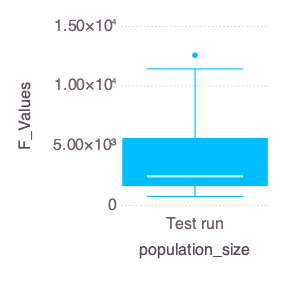
\includegraphics[scale=0.6]{../data/Plots/comparation.png}
	\caption{Ejecución para probar la librería \emph{GeneticAlgorithms.jl}. Se ha ejecutado para un tamaño de población de 100. Como función de fitness Rastrigin.}
    \label{fig:genetic_algorithms_jl}
\end{figure}


	
	\chapter{Planificación y metodología utilizada}

En este capítulo se comentará la planificación del proyecto y la metodología usada. La metodología
es muy importante para este TFG, ya que uno de los objetivos es desarrollar siguiendo una metodología
ágil.

\section{Metodología utilizada}

Un requisito fundamental a la hora de la implementación es usar una metodología que garantice la evolución del código,
dado que está definido como uno de los objetivos del TFG. Por eso se ha elegido usar el desarrollo ágil, específicamente 
la metodología Kanban. Este método tiene 4 principios básicos \cite{kanban}:

\begin{itemize}
    \item Empezar con lo que se hace ahora: no es necesario realizar cambios drásticos para empezar a utilizarlo.
    \item Comprometerse a buscar e implementar cambios incrementales y evolutivos: se trata de definir las tareas
    pensando en cuál sería el mínimo esfuerzo que se puede realizar en la tarea, pero que aún así aporte valor al producto final.
    Consiste pues en pequeños y continuos cambios incrementales y evolutivos del proceso actual.
    \item Lo siguiente a realizar se decide del backlog (tareas pendientes acumuladas), pudiéndose priorizar aquellas 
    tareas entrantes según las necesidades del momento.
    \item  En el Kanban no se premia la rapidez, sino la calidad del producto final.
\end{itemize}

Se ha decidido usar esta metodología, debido a que es muy flexible a los cambios que se puedan producir a lo largo del proyecto. Esto va en
línea con el objetivo de usar metodología ágil durante el desarrollo del proyecto, además es parte de los requisitos no funcionales del proyecto \ref{sect:no-funcionales}

En cuanto al desarrollo del código se ha elegido la metodología de desarrollo guiado por pruebas o \emph{TDD}. Este método
de desarrollo encaja muy bien con Kanban, porque para cada tarea que se finalice tienes una funcionalidad completa y testeada. De esta manera, la mantenibilidad del código aumenta, y al final del desarrollo te aseguras de que todas las piezas funcionan. Otra cualidad de
este tipo de desarrollo es que los tests ayudan mucho a las personas que usen la librería por primera vez, ya que se puede 
ir probando la funcionalidad fácilmente. Además, estas pruebas pueden servir como documentación, ya que en los tests se ve claramente 
los parámetros de entrada y de salida de la función. El TDD consiste en:

\begin{itemize}
    \item \textit{Escritura del test} - escribir el test que cubra la funcionalidad que se va a desarrollar.
    \item \textit{Fallo del test} - dado que aún no hemos codificado esa funcionalidad, el test debe fallar.
    \item \textit{Escribir código para pasar el test} - escribir el mínimo código posible para que el test pase.
    \item \textit{Refactorizar el código} - añadir lo necesario para seguir completando la funcionalidad.
    \item \textit{Repetir} - los pasos anteriores hasta completar la funcionalidad.
\end{itemize}

Los tests que se vayan realizando se usarán para la integración continua del proyecto o \emph{CI}.
La integración continua se refiere en su mayoría a la fase de creación o integración del proceso de publicación de
software y conlleva un componente de automatización \cite{CI}. Tener integración continua en el proyecto hace que sea
mantenible, ya que se protege ante cambios. Siempre que hagas cambios, si los tests pasan te da seguridad de que tu cambio se 
acopla bien a la funcionalidad antigua. 


\section{Herramientas de comunicación}

Para llevar el desarrollo del proyecto se ha utilizado la plataforma GitHub, donde se encuentra todo lo 
relacionado con el trabajo \cite{project_repository}. Esta plataforma posibilita un desarrollo cómodo gracias a la cantidad
de herramientas que provee. Para las historias de usuario se han usado los \textit{issues}; para tener una
visión general del estado del proyecto se ha usado \textit{Projects}, que permite añadir columnas. Siguiendo el método Kanban, el
tablero tiene 3 columnas, la tarea más prioritaria sería la que está más arriba a la derecha:

\begin{itemize}
    \item \emph{Product Backlog}: contiene todas las tareas que se quieren desarrollar, priorizadas de manera que la más urgente
    se encuentre la primera en la columna.
    \item \emph{In progress}: contiene todas las tareas que están abiertas en el momento. Siguiendo Kanban esta columna
    debe tener siempre el mínimo de tareas posibles. La prioridad es siempre cerrar tareas antes de empezar una nueva.
    \item \emph{Done}: contienen las tareas que ya se han finalizado.
\end{itemize}

Cada tarea del \emph{backlog} tiene un \emph{pull request} enlazado, ya que cada tarea es un requisito del producto final. Todo
esto se encuentra en un repositorio público. Cualquiera puede añadir nuevas tareas al proyecto y puede ver el progreso realizado en ellas.
Facilita mucho la corrección al tutor, ya que puede comentar cualquier línea de código y crear una tarea pidiendo alguna
modificación. Además, Github se integra con Telegram a través de un bot, y por cada cambio que hace al proyecto se envía un mensaje
a un grupo en el que estamos el tutor del trabajo y yo. Este mensaje contiene un enlace al cambio que se ha hecho. Consecuentemente,
es sencillo llevar un seguimiento exhaustivo de todo lo que pasa en el repositorio.

\section{Casos de uso} \label{sect:use_cases}

En línea con el tercer objetivo de aplicar desarrollo ágil en la ciencia, el proyecto se ha desarrollado definiendo
historias de usuario, definidas usando \emph{Desarrollo basado en el comportamiento} o BDD \cite{BDD}. Lo que 
plantea BDD es definir un lenguaje común para todas las partes implicadas en un proyecto, y utilizar esto como parte inicial 
del desarrollo y el testeo. Todas las historias están en el repositorio de Github del proyecto \cite{project_repository}.
Las historias se pueden dividir en 2 grandes grupos o épicas: definir la funcionalidad básica y análisis de los resultados.

En el caso de la funcionalidad básica se encuentran las siguientes historias de usuario, con el enlace al
\emph{issue} y su correspondiente \emph{pull request}:

\begin{enumerate}
    \item \textbf{Sistema de entrada de la biblioteca} \label{it:sist_entrada}: Como desarrolladora quiero tener una forma de leer ficheros de configuración de forma que pueda
    establecer los datos leídos como los parámetros iniciales del algoritmo. Los parámetros a definir por el usuario son: la dimensión del cromosoma, el tamaño de la población, 
    la condición de parada basado en el número máximo de generaciones que puede estar el algoritmo sin producir mejores soluciones, el porcentaje de la población que va a cada casta y 
    el tasa de mutación que tendrán los individuos de cada casta.
    \item \textbf{Función de fitness \cite{project_repository_8}} \label{it:fitness_function}: Como desarrolladora quiero tener distintas funciones fitness disponibles de manera que pueda aplicarlas según 
    el problema.
    \item \textbf{Sala de fecundación \cite{project_repository_17}}: como desarrolladora quiero tener una sala de fecundación de manera que la población sea dividida en castas siguiendo los parámetros establecidos
    en el fichero de configuración.
    \item \textbf{Definir las castas como tipos \cite{project_repository_21}}: como desarrolladora quiero tener las castas definidas como tipos para poder explotar el \emph{dispatch} múltiple en los operadores de evolución.
    \item \textbf{Operador de selección \cite{project_repository_18}} \label{it:selection_operator}: como desarrolladora quiero tener un operador de selección de manera que los mejores individuos sean seleccionados para la reproducción.
    \item \textbf{Operador de cruce \cite{project_repository_19}} \label{it:crossover_operator}: como desarrolladora quiero tener un operador de cruce de manera que pueda obtener un nuevo individuo dados dos padres.
    \item \textbf{Operador de mutación \cite{project_repository_20}} \label{it:mutation_operator}: como desarrolladora quiero tener un operador de mutación, de manera que pueda mutar los genes de un cromosoma atendiendo al parámetro
    \emph{``tasa de mutación``} dado por el fichero de configuración. 
\end{enumerate}

Para el análisis de los resultados, una vez definidos los datos que se quieren recoger en cada generación \cite{pull_17}, 
se guardarán en ficheros que se leerán para imprimir las gráficas.

Todos estos componentes conforman lo que sería el producto mínimamente viable o \emph{MVP} del TFG. El MVP es un producto
con suficientes características para satisfacer a los clientes iniciales, y proporcionar retroalimentación para el desarrollo futuro \cite{mvp}. 
Este concepto se alinea con la metodología ágil, ya que se trata de presentar lo mínimo que pueda usarse. A partir de ahí se puede mejorar 
añadiéndole, por ejemplo, paralelismo. De esto se hablará en secciones posteriores.


	% Desarrollo bajo sprints: 
	% 	1. Permitir registros y login de usuarios
	% 	2. Desarrollo del sistema de incidencias
	% 	3. Desarrollo del sistema de denuncias administrativas y accidentes
	% 	4. Desarrollo del sistema de croquis
	%   5. Instalación de la aplicación de manera automática
	\chapter{Implementación}
En esta sección se va a describir la implementación, basada en los requisitos mencionados.

\section{Lenguaje de programación}

Una de las formas de conseguir altas prestaciones, para alcanzar el objetivo 2, es escoger el lenguaje adecuado. Por ello se ha elegido
un lenguaje que hace poco entró en el \"Petaflop Club\", el cual incluye aquellos lenguajes que superan 1 petaflop/segundo como rendimiento pico. Se trata
de Julia \cite{julia}, un lenguaje de programación multiparadigma de tipado dinámico. Orientado a la computación técnica y
científica, el objetivo de sus creadores fue el de combinar lo mejor de otros lenguajes, es decir, conseguir un “todo en uno”, lo que se traduce en:
la velocidad de C, la usabilidad de Python, el dinamismo de Ruby, la destreza matemática de MatLab, y las estadísticas de R \cite{julia_goals}.

\section{Metodología del desarrollo}

Un requisito fundamental a la hora de implementar es usar una metodología que garantice la evolución del código. Por eso la implementación 
del software se ha dividido en tareas, siguiendo la metodología ágil Kanban. Se divide pues el proyecto en tareas pequeñas que aporten valor al producto 
final, de esta forma que puedes probar cada tarea a medida que la vas acabando. Al final del desarrollo estás segura de que todas las piezas funcionan
correctamente.

Otro requisito es desarrollar un algoritmo que sea mantenible. Por tanto, a la hora del desarrollo se priorizarán conceptos 
como arquitectura limpia \cite{cleanArquitecture2017} y la limpieza del código \cite{cleanCode2008}, así como el desarrollo basado en tests. De esta manera, se asegura
que el algoritmo está asentado sobre una base firme. Asimismo, gracias al desarrollo basado en tests, para cada cambio que se haga
se sabrá si se ha roto lo que estaba escrito hasta el momento.  Usar estándares va en línea con el objetivo de aplicar el desarrollo ágil a la ciencia.

\section{Estructuras de datos}

Las entidades que se han utilizado para estructura la información son:
\begin{itemize}
    \item Para tener bien definidos los datos de entrada se ha creado una entidad que contiene todos los parámetros de
    configuración del algoritmo. Se trata de una estructura inmutable, luego estos parámetros no cambiarán a lo largo de todo el
    algoritmo.
    \item Para unificar todos los datos que necesita el algoritmo, se ha definido una estructura inmutable. Una vez
    rellenada esta entidad, el algoritmo tiene todos los datos necesarios para comenzar la ejecución.
    \item Definir la casta como una entidad abstracta. Julia usa el \emph{dispatch} múltiple como paradigma, 
    lo que va a ser muy útil a la hora de definir los operadores, como se verá más adelante. Teniendo la casta 
    como tipo abstracto podremos definir métodos que acepten cualquier tipo de casta.

    \item Julia es un lenguaje de tipado dinámico, pero tiene alguna de las ventajas del tipado estático, haciendo posible indicar
    los tipos de algunos valores. Además, para poder hacer buen uso de este paradigma se han definido las castas como tipos distintos, por ejemplo, para
    la casta alfa:

    \begin{lstlisting}[
        basicstyle=\small
    ]
        @with_kw struct ALPHA <: Caste
            name::String = "ALPHA"
        end
    \end{lstlisting}

    El decorador \lstinline{with_kw} de la biblioteca \emph{Parameters.jl}, para poder añadir parámetros por defecto a una entidad. Las castas se han definido 
    como tipos inmutables, ya que en ningún momento se va a cambiar el nombre propio de la casta.
\end{itemize}

\section{Implementación de los casos de uso}

En esta sección se va a describir las decisiones técnicas que se han tomado para desarrollar los casos de uso \ref{sect:use_cases}

\begin{itemize}
    \item \textbf{Sistema de entrada de la biblioteca} \ref{it:sist_entrada}: usar el formato JSON para definir los parámetros
    del algoritmo. Un ejemplo de fichero sería el siguiente:
    \begin{lstlisting}[
        basicstyle=\small
    ]
        {
            "CHROMOSOME_SIZE": 2,
            "POPULATION_SIZE": 100,
            "MAX_GENERATIONS": 15,
            "POPULATION_PERCENTAGE": {
                "ALPHA": 10,
                "BETA": 20,
                "GAMMA": 20,
                "DELTA": 20,
                "EPSILON": 30
            },
            "MUTATION_RATE": {
                "ALPHA": 10,
                "BETA": 10,
                "GAMMA": 10,
                "DELTA": 10,
                "EPSILON": 10
            }
        }
    \end{lstlisting}

    Cualquiera de estos parámetros se puede cambiar. Esto se convertirá en una entidad inmutable que servirá como 
    entrada al algoritmo.

    \item \textbf{Función de fitness \cite{project_repository_8}}: se han usado las funciones que pertenecen al \emph{benchmark}
    \emph{ Black-box Optimization Benchmarking (BBOB)} \cite{bbob_definition}. Este \emph{benchmark} define funciones que se suelen 
    usar como referencia en el campo de las metaheurísticas. En Julia están implementadas en la biblioteca 
    \emph{BlackBoxOptimizationBenchmarking.jl} \cite{bbob_jl}.

    \item \textbf{Operadores de selección, cruce y mutación} [\ref{it:selection_operator}, \ref{it:crossover_operator}, \ref{it:mutation_operator}]:
    Se ha usado el \emph{dispatch} múltiple para definir operadores que se adecúen en cada casta. Por ejemplo, para el caso del
    operador de selección se han definido 3 tipos de parámetros de entrada:

    \begin{lstlisting}[
        basicstyle=\small
    ]
        selector_operator(
            caste::ALPHA, 
            caste_population
        )
        selector_operator(
            caste::BETA, 
            caste_population, 
            alpha_reproduction_pool
        )
        selector_operator(
            caste, 
            caste_population
        )
    \end{lstlisting}
    
    Para muestrear la población se ha usado la biblioteca \emph{StatsBase.jl}. Se ha elegido esta librería porque
    tiene un gran número de contribuidores y se actualiza continuamente.
\end{itemize}

\section{Implementación del cálculo de la diversidad}

Uno de los objetivos del TFG es mejorar la diversidad en problemas de optimización mediante la división de la población en castas.
Para calcularla se han usado como métricas la entropía y la distancia de edición; la decisión de usar estas medidas
está definida en secciones posteriores. Para calcular la entropía en Julia hay varias librerías disponibles:

\begin{itemize}
    \item \emph{Entropy.jl} \cite{entropy_jl}: este paquete contiene funcionalidad para ejecutar estimaciones de la entropía. No se ha usado porque,
    aparte de no tener nada de documentación, la última vez que se actualizó fue hace 8 años, por tanto contiene
    sintaxis antigua que no compilará con las nuevas versiones del lenguaje.
    \item \emph{Diversity.jl} \cite{diversity_jl}: este paquete provee de funcionalidad para calcular diferentes
    tipos de diversidad. Es una biblioteca muy completa, pero tiene una curva de aprendizaje muy grande, ya que los
    operadores definidos para el cálculo son muy teóricos. Además no tiene para calcular la entropía y la distancia
    de edición.
\end{itemize}

Al final para calcular la entropía se ha usado el paquete \emph{InformationMeasures.jl} \cite{informationMeasures_jl}, ya 
que tiene una función que te calcula la entropía para cualquier tipo de datos. Aparte, ha sido muy fácil usarla porque 
tiene buena documentación. La distancia de edición a partir de la distancia euclídea ofrecida por el paquete
\emph{Distances.jl} \cite{distances_jl}, paquete que ofrece gran cantidad de opciones para calcular distancias entre vectores.
Para calcular distancias era una de las pocas opciones disponibles, pero tiene muchos contribuidores, ya que forma 
parte de paquetes Julia Statistics \cite{stats_jl}.

\section{Implementación necesaria para el análisis de los resultados}

Para el análisis de los resultados se ha usado la estructura de datos \emph{DataFrames}, del paquete \emph{Dataframes.jl}. Se
ha usado esta estructura de datos porque facilita mucho la visualización en tablas. Además tiene una fuerte
integración con distintos formatos de salida de archivos. 

Para las gráficas se usará \emph{Gafly.jl} \cite{gadfly_jl},ya que se integra estrechamente con los DataFrames.


	% Análisis del problema
	% 1. Análisis de requisitos
	% 2. Análisis de las soluciones
	% 3. Solucion propuesta
	% 4. Análisis de seguridad
	\chapter{Análisis del problema}

\section{Diversidad}

Recordemos que el objetivo 1 de este trabajo era mejorar la diversidad en problemas de optimización mediante la división de la población en castas.
Mantener la diversidad es crucial para evitar una convergencia prematura hacía un óptimo local. Rosca \cite{Rosca} concluyó que las poblaciones parecían quedar estancadas
en un óptimo local cuando la entropía no cambiaba o decrecía monótonamente en las generaciones sucesivas. En programación genética, la diversidad se refiere a diferencias estructurales, 
como por ejemplo la cantidad de genotipos distintos en la población o la singularidad de valores del fitness \cite{genetic}. Uno de los objetivos de este trabajo es investigar cómo la 
división en castas afecta a la diversidad, así que en esta sección se analizará.  Hay diferentes medidas para calcularla, entre ellas: diversidad genotípica, 
diversidad fenotípica, entropía, pseudo-isomorfismo, distancias de edición, etc. De entre ellas calcularemos la \textbf{entropía}, que describe cómo se distribuye la
población en torno a los diferentes valores del fitness, y la \textbf{distancia de edición}, en la que cada individuo se mide contra el mejor individuo encontrado hasta el 
momento. Se han elegido dado que según Burke \cite{diversity} la entropía y la distancia de edición muestran una gran correlación con el aumento y decremento del valor 
del fitness. Una vez calculadas, se investigará la relación entre el fitness y la diversidad \cite{diversity}. 

\subsection{Experimentos}

Para realizar estas pruebas usaremos la configuración de la Tabla \ref{tab:diversity_config}, como función a minimizar la función Rastrigin \cite{BBOB}, y la distancia euclídea.

\begin{table}[]
    \centering
    \begin{tabular}{||c|c||}
        \hline
        \multicolumn{2}{|l|}{\textbf{Fichero Configuración: config\_file\_5.json} \ref{subsect:config_file_5}} \\ \hline
        Tamaño del cromosoma                            & 20              \\ \hline
        Tamaño de la población                          & 100             \\ \hline
        Máximo de generaciones                          & 15              \\ \hline
        Porcentaje Alfa de la población                 & 10              \\ \hline
        Porcentaje Beta de la población                 & 20              \\ \hline
        Porcentaje Gamma de la población                & 20              \\ \hline
        Porcentaje Delta de la población                & 20              \\ \hline
        Porcentaje Epsilon de la población              & 30              \\ \hline
        Tasa de mutación                               & 10              \\ \hline
    \end{tabular}
    \caption{Parámetros de configuración para exploración de la diversidad}
    \label{tab:diversity_config}
\end{table}

\begin{figure}[H]
	\centering	
	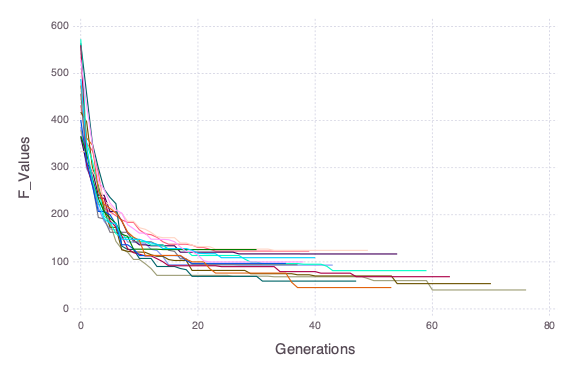
\includegraphics[scale=0.6]{../data/Plots/config_file_5_Rastrigin.png}
	\caption{Primera ejecución}
    \label{fig:primera_ejecucion}
\end{figure}

En la Figura \ref{fig:primera_ejecucion} se ve el resultado de ejecutar el algoritmo 15 veces con la configuración anterior.
Se puede observar cómo los mejores resultados se obtienen en las primeras generaciones. La mayoría de las ejecuciones muestran cómo la mejora
del fitness disminuye alrededor de la generación 15-20. Esto puede indicar que cuanto mayor es la generación menor es la diversidad. 
Para apoyar esta idea tenemos las Figuras \ref{fig:best_f_value} y \ref{fig:worst_f_value}. 

La Figura \ref{fig:best_f_value} muestra la diversidad de la ejecución que resulta en un mejor fitness. De la generación 0 a la 30 se produce un decremento de la entropía,
pero se vuelve a recuperar en el resto de generaciones. La entropía empezando y acabando casi con el mismo valor nos dice que el algoritmo mantiene una diversidad similar a 
lo largo de toda la ejecución, lo que puede dar lugar a mejores resultados. En la Figura \ref{fig:worst_f_value}, que muestra la peor ejecución, podemos 
ver un comportamiento similar; el descenso también se produce en las generaciones 0-25. 

\begin{table}[]
    \begin{tabular}{||c|c|c|c|c|c||}
    \hline
                                                                            & \textbf{\begin{tabular}[c]{@{}c@{}}Evals. de \\ f\end{tabular}} & \textbf{Entropía} & \textbf{\begin{tabular}[c]{@{}c@{}}Distancia de \\ edición\end{tabular}} & \textbf{Mejor f} & \textbf{Generaciones} \\ \hline
    \textbf{\begin{tabular}[c]{@{}c@{}}Mejor \\ ejecución\end{tabular}}     & 11873                & 2.69              & 6.20                          & 40.27                     & 77                    \\ \hline
    \textbf{\begin{tabular}[c]{@{}c@{}}Peor \\ ejecución\end{tabular}}      & 4900                 & 2.11              & 5.95                          & 126.14                    & 31                    \\ \hline
    \end{tabular}
    \caption{Comparación de la ejecución con mejor valor de fitness y la peor, usando el fichero de configuración 5 [\ref{subsect:config_file_5}]}
    \label{fig:Comparación}
\end{table}

En ambas imágenes la distancia de edición mantiene una correlación estrecha con el valor del fitness, y en ambos casos acaba con unos valores similares. Mirando la tabla \ref{fig:Comparación}, y las figuras
mencionadas no se puede concluir una diferencia clave que marque el por qué una es la mejor ejecución y otra la peor.

\begin{figure}[]
	\centering	
	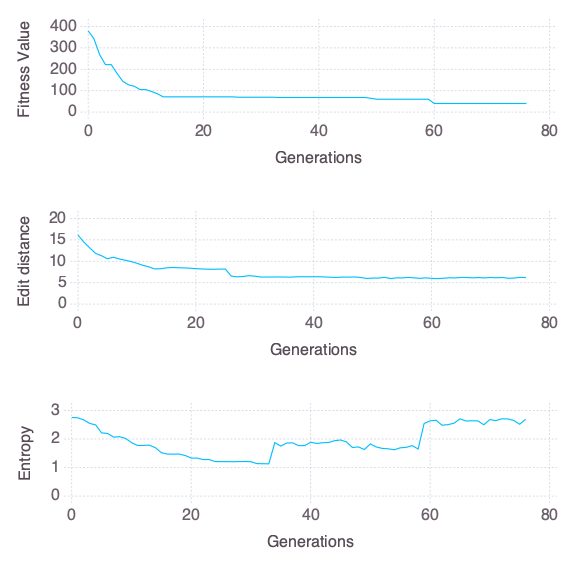
\includegraphics[scale=0.5]{../data/Plots/config_file_5_Rastrigin_best_f_value.png}
	\caption{ Diversidad en la ejecución con mejor resultado de fitness }
    \label{fig:best_f_value}
\end{figure}

\begin{figure}[]
	\centering	
	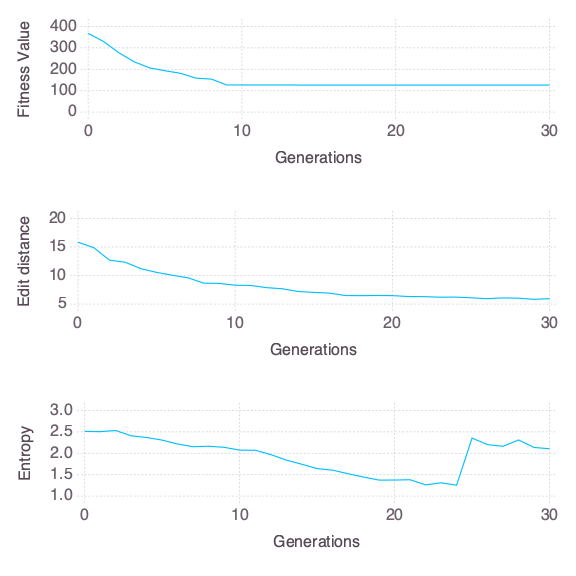
\includegraphics[scale=0.5]{../data/Plots/config_file_5_Rastrigin_worst_f_value.png}
	\caption{ Diversidad en la ejecución con peor resultado de fitness }
    \label{fig:worst_f_value}
\end{figure}

\section{Exploración Inicial}

El objetivo de esta exploración es escoger los parámetros: dimensión del cromosoma (\textit{DIM}) y tamaño de población. Primero se varía la dimensión
del cromosoma y la población se mantiene fija a 100. Se ejecutará el algoritmo 15 veces por cada dimensión del cromosoma, y se cogerá el que 
tenga mejor resultado para la comparación. Los resultados de esta primera exploración se encuentran en la Tabla \ref{tab:fitness_variation}. 

\begin{table}[]
    \centering
    \begin{tabular}{||c|c|c|c|c|c||}
        \hline
        \textbf{Fichero Configuración} & \textbf{Generaciones} & \textbf{DIM} & \textbf{Mejor fitness} & \textbf{Evals. de f}\\ \hline
        Config 1   & 16    & 2   & -76.93    &  2340  \\ \hline
        Config 2   & 20    & 3   & -74.70    &  2900  \\ \hline
        Config 3   & 20    & 5   & -67.58    &  2900  \\ \hline
        Config 4   & 56    & 10  & -45.74    &  8567  \\ \hline
        Config 5   & 68    & 20  & 49.43     &  10494 \\ \hline
        Config 6   & 52    & 40  & 422.26    &  8133  \\ \hline
    \end{tabular}
    \caption{Resultados exploración inicial}
    \label{tab:fitness_variation}
\end{table}

\begin{figure}[]
	\centering	
	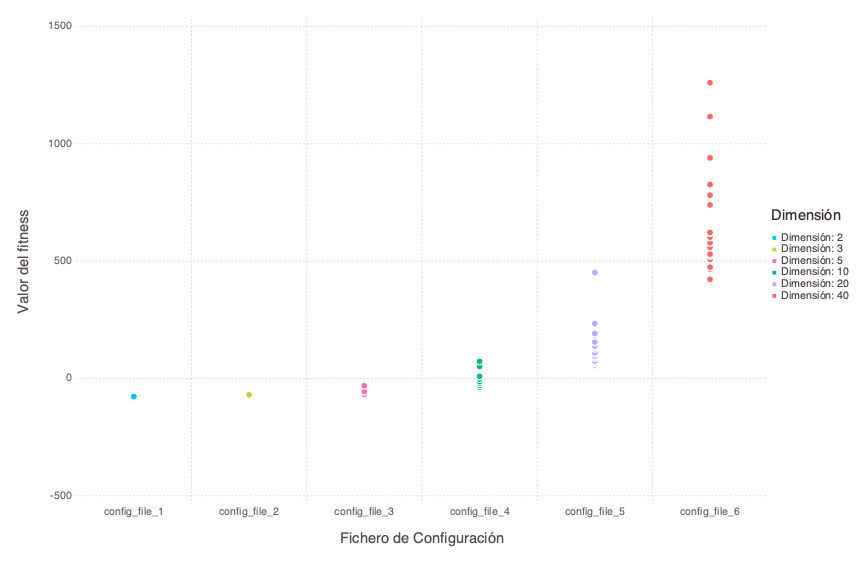
\includegraphics[scale=0.4]{figuras/config_file_1-6_Rastrigin_box_plots.png}
	\caption{ Variación del valor del fitness }
    \label{fig:box_plots}
\end{figure}

Para un tamaño de población 100 aparentemente la mejor dimensión es la 3. Sin embargo, mirando la Figura \ref{fig:box_plots} vemos
que la configuración 2 apenas ha explorado el espacio, ha alcanzado un óptimo local, al igual que de la 1 a la 3. Para
futuras explotaciones descartaremos estas configuraciones, ya que no aportan apenas información sobre el comportamiento del algoritmo.
Con la información extraída de estos experimentos no se puede concluir qué valores escoger para el tamaño de población ni para la
dimensión del cromosoma escoger. En las siguientes secciones se le dará un enfoque diferente.
\section{Exploración del tamaño de población}

\begin{table}[]
    \centering
    \begin{tabular}{|c|c|c|c|c|c|}
        \hline
        \textbf{Config.} & \textbf{\begin{tabular}[c]{@{}c@{}}Tmñ.\\ Población\end{tabular}} & \textbf{\begin{tabular}[c]{@{}c@{}}Mediana \\ mejor valor \\ de fitness\end{tabular}} & \textbf{\begin{tabular}[c]{@{}c@{}}Mediana \\ \# ejecuciones \\ de f\end{tabular}} & \textbf{\begin{tabular}[c]{@{}c@{}}$\sigma$\\ mejor valor\\ de fitness\end{tabular}} & \textbf{\begin{tabular}[c]{@{}c@{}}$\sigma$\\ \# ejecuciones \\ de f\end{tabular}} \\ \hline
        4  [\ref{subsect:config_file_4}]                & 100                                                               & 7.00                                                                                  & 7852.0                                                                             & 11.98                                                                         & 2045.87                                                                     \\ \hline
        7  [\ref{subsect:config_file_7}]                & 150                                                               & 0.27                                                                                  & 9010.0                                                                             & 15.10                                                                         & 2536.42                                                                     \\ \hline
        8  [\ref{subsect:config_file_8}]                & 300                                                               & -18.06                                                                                & 23496.0                                                                            & 10.20                                                                         & 6406.70                                                                     \\ \hline
        9  [\ref{subsect:config_file_9}]                & 500                                                               & -26.11                                                                                & 37087.0                                                                            & 5.61                                                                          & 8492.77                                                                     \\ \hline
        10 [\ref{subsect:config_file_10}]               & 1000                                                              & -33.53                                                                                & 75539.5                                                                            & 5.63                                                                          & 21178.32                                                                    \\ \hline
    \end{tabular}
    \caption{Resultados exploración inicial para diferentes tamaños de población}
    \label{tab:base_population}
\end{table}

El objetivo de esta sección es obtener una población inicial base para las próximas exploraciones. Dejaremos fija la dimensión del cromosoma a 10 y
ejecutaremos cada fichero de configuración 15 veces. Se ha escogido esta dimensión porque ha alcanzado una solución 
relativamente buena en el experimento anterior. Las soluciones de esta exploración se encuentran en la Tabla \ref{tab:base_population}. 
En esta nueva exploración se han probado los tamaños de población: 100, 150, 300, 500, 1000, indicados en la Tabla \ref{tab:base_population}
como \textit{Tmñ. poblacion}. En la Figura \ref{fig:population_size_variation} se vuelve a ver cómo el mayor descenso del valor del fitness se produce
entre la generación 0 y la 20. La población con tamaño 1000 (Config 10 en Tabla \ref{tab:base_population}) es la que tiene
un mayor descenso pasada la generación 20. 

\begin{figure}[]
	\centering	
	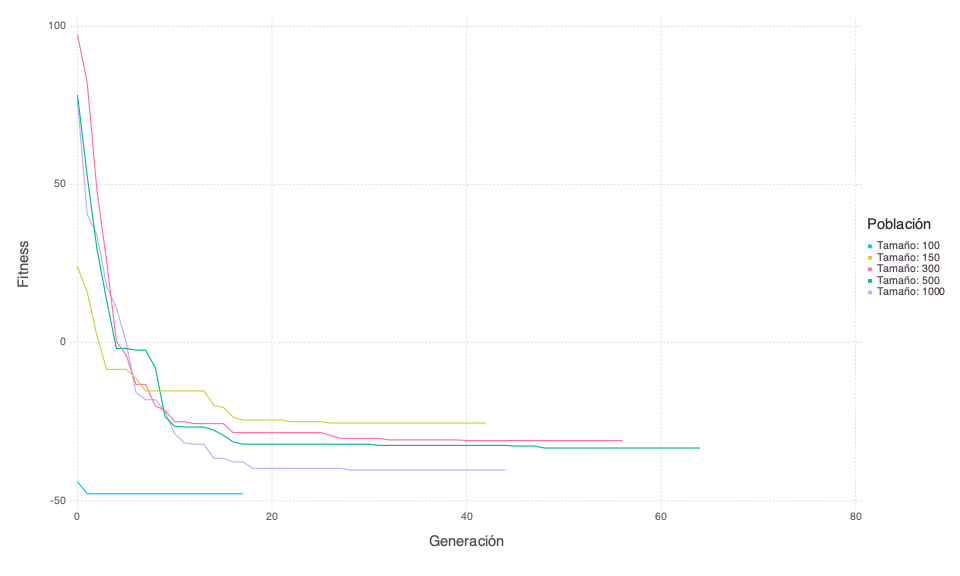
\includegraphics[scale=0.5]{../data/Plots/population_size_variation.png}
	\caption{ Ejecuciones variando el tamaño de la población }
    \label{fig:population_size_variation}
\end{figure}

En la Figura \ref{fig:population_size_box_plots}, se ve que la configuración 4 [\ref{subsect:config_file_4}] es la que alcanza un valor más pequeño de fitness.
Sin embargo mirando la Tabla \ref{tab:base_population} es la configuración 10 [\ref{subsect:config_file_10}] la que tiene mejor mediana para el valor del 
fitness, y además menor desviación típica, por lo que en general se mueve por solciones relativamente buenas.

\begin{figure}[]
	\centering	
	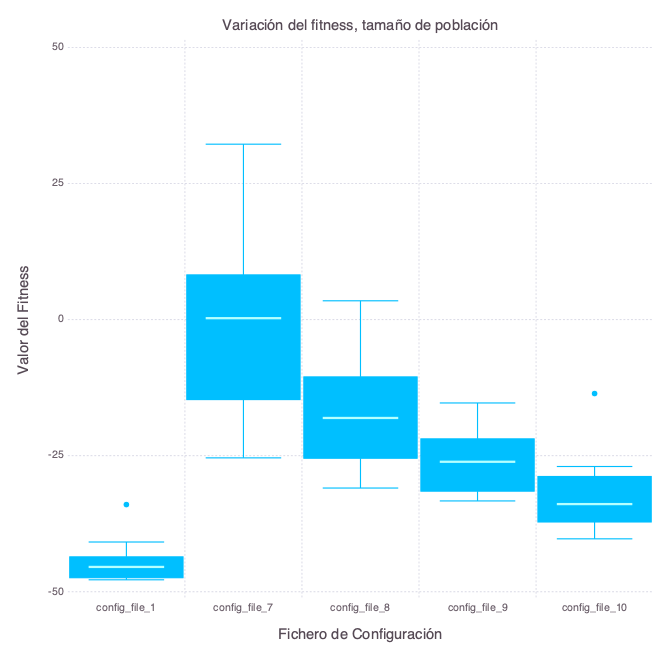
\includegraphics[scale=0.5]{../data/Plots/Rastrigin_box_plots_p_size.png}
	\caption{ Diversidad en la ejecución variando el tamaño de población }
    \label{fig:population_size_box_plots}
\end{figure}


El objetivo de esta exploración era sacar una población inicial en la que basar el resto de experimentos. Por tanto atendiendo al que tiene mejor mediana,
usaremos la configuración 10 [\ref{subsect:config_file_10}] para las siguientes exploraciones.


\section{Análisis de las soluciones}

- en que casos da mejor resultado y por qué, comparar con hipótesis inicial
- Por qué da mejores resultados con una función o con otra o con respecto al algoritmo genético


\section{Comparación con GeneticAlgorithms.jl}


	% Presupuesto

	% Conclusiones
	\chapter{Conclusiones}



	% Trabajos futuros
	\chapter{Trabajos Futuros}

	\newpage
	\bibliography{bibliografia}
	\bibliographystyle{plain}
	
\end{document}

